\documentclass[11pt,a4paper]{report}
\usepackage[margin=1in]{geometry}
\usepackage{amsmath,amssymb,amsthm,mathtools}
\usepackage{booktabs,array,tabularx}
\usepackage{tikz}
\usetikzlibrary{arrows.meta,positioning,calc,fit,backgrounds,shapes.geometric}
\usepackage[hidelinks]{hyperref}
\usepackage{microtype}
\usepackage{xcolor}
\usepackage{graphicx}
\usepackage{listings}
\usepackage{enumitem}
\usepackage{caption}

\definecolor{ran}{HTML}{2B6CB0}
\definecolor{tra}{HTML}{2F855A}
\definecolor{core}{HTML}{B7791F}
\definecolor{svc}{HTML}{805AD5}
\definecolor{ink}{HTML}{222222}
\definecolor{rule}{HTML}{BBBBBB}

\lstset{basicstyle=\ttfamily\small,columns=fullflexible,keepspaces=true,frame=single,rulecolor=\color{rule},breaklines=true}

\newtheorem{definition}{Definition}[chapter]
\newtheorem{proposition}{Proposition}[chapter]
\newtheorem{remark}{Remark}[chapter]
\newtheorem{assumption}{Assumption}[chapter]

\newcommand{\R}{\mathbb{R}}
\newcommand{\V}{\mathcal{V}}
\newcommand{\E}{\mathcal{E}}
\newcommand{\Rel}{\mathcal{R}}
\newcommand{\Tset}{\mathcal{T}}
\newcommand{\N}{\mathcal{N}}
\newcommand{\Sym}{\mathrm{Sym}}
\newcommand{\norm}[1]{\left\lVert #1 \right\rVert}
\newcommand{\ind}[1]{\mathbf{1}\!\left[#1\right]}
\newcommand{\code}[1]{\texttt{#1}}

\title{\vspace{-2em}\textbf{The Geometry of Network Healing}\\[0.4em]
\large Geometric deep learning for business-aware, self-healing telecom networks\\[0.3em]
\normalsize Open mathematics, open code, NVIDIA-accelerated \quad\textperiodcentered\quad branch: edge-ai-grid}
\author{David Kypuros}
\date{October 2026 \quad\textperiodcentered\quad v0.1}

\begin{document}
\maketitle

\begin{abstract}
\noindent
A telecom network is not a grid. It is a heterogeneous directed graph whose node labels carry no
information, whose faults propagate along typed dependency edges, and whose business value is
concentrated in a few revenue-dense cells. This monograph derives, from the geometric deep learning
blueprint, the minimal learning system that detects silent degradation without alarms, ranks root
causes across RAN, Core and Transport from one service-layer trigger, and orders remediation by
revenue at risk under a resource budget. Every numbered equation maps to a module in the
accompanying open-source repository, and every claim is measured on a synthetic digital twin with
injected faults against graph-free baselines. The point is simple: the model is mathematics anyone
can implement; the operator's moat is the topology and the history, not the network.
\end{abstract}

\tableofcontents

\chapter{The claim}
\label{ch:claim}

\section*{Same fault, different response}
Two cells degrade by the same amount. One carries a stadium on match day; the other carries a
car park at 3\,a.m. Today both enter the same resolution queue because the network has no
vocabulary for the difference. Cross-domain triage, deciding whether a service-layer symptom
comes from the radio, the transport ring or the core, is still largely a human walking three
dashboards.

Recent industry work on autonomous networks has shown that a graph neural network over a temporal
digital twin, with a business-intent layer on top and standards-based orchestration below, can
close that loop at Level~4 autonomy. The public descriptions of such systems are impressive and
also, on inspection, built from three ingredients:

\begin{enumerate}[nosep]
  \item a graph database that holds the topology and its history (engineering);
  \item a graph neural network that reads the topology and the KPI history (mathematics);
  \item an intent vocabulary that lets business priority reorder remediation (a small optimisation).
\end{enumerate}

Items 2 and 3 are not proprietary. They are consequences of a general blueprint, geometric deep
learning~\cite{bronstein2021}: identify the symmetry group of your domain, build layers that respect
it, pool locally, read out invariantly. This document does that derivation for a telecom network,
writes down every operator, implements it in open code, and measures it. Item~1 is real engineering
at operator scale and is discussed honestly in Chapter~\ref{ch:nvidia}, where we describe the NVIDIA
path (GPU-resident graph storage with WholeGraph, GPU sampling with cuGraph-PyG) that we assume for
scale-out.

\section*{What is and is not claimed}
\begin{itemize}[nosep]
  \item \textbf{Claimed.} The learning stack of a business-aware GNN-healing system is reproducible
  from the equations in Chapters~\ref{ch:domain}--\ref{ch:intent} by anyone with the topology and the
  KPI history. Our implementation detects injected silent degradations earlier than static-threshold
  alarms, ranks the true origin first in the large majority of episodes, and changes the remediation
  order when revenue changes (Chapter~\ref{ch:experiments}).
  \item \textbf{Not claimed.} That the synthetic twin is a real network. Its purpose is to be
  \emph{falsifiable}: every number in Chapter~\ref{ch:experiments} is produced by one command from a
  fixed seed, and the generator and fault model are the first thing a reader should change.
  \item \textbf{Not claimed.} Any particular vendor's results. No proprietary data or code is used.
\end{itemize}

\section*{How to read this}
Each chapter ends in numbered equations. Appendix~\ref{app:map} maps every equation to the Python
module that implements it. Chapter~\ref{ch:experiments} is generated from the repository's
\code{results/results.md}. If you change an equation, change the module, rerun, and the table changes.

\chapter{The domain}
\label{ch:domain}

\section{A network as a heterogeneous directed graph}
\begin{definition}[Network graph]
A network is a tuple $G=(\V,\E,\tau,\rho)$ where $\V$ is a finite set of $N$ nodes,
$\E\subseteq\V\times\V$ a set of directed edges, $\tau:\V\to\Tset$ a node-type map and
$\rho:\E\to\Rel$ an edge-relation map.
\begin{equation}
G=(\V,\E,\tau,\rho),\qquad
\Tset=\{\textsf{cell},\textsf{gnb},\textsf{router},\textsf{link},\textsf{upf},\textsf{amf},\textsf{smf},\textsf{service}\}.
\label{eq:graph}
\end{equation}
\end{definition}

Three choices in \eqref{eq:graph} matter and are easy to get wrong.

\paragraph{Edges point in the direction a fault propagates.} An edge $v\to u$ means ``a
degradation at $v$ is felt at $u$''. A fibre link feeds a router; a core router feeds an aggregation
router; an aggregation router backhauls a gNB; a gNB serves cells; the AMF controls gNBs; the SMF
controls UPFs; a core router feeds a UPF; a UPF terminates services; cells carry services. This
is the \emph{causal} orientation, not the traffic orientation, and it is what makes
Chapter~\ref{ch:propagation} a diffusion and Chapter~\ref{ch:inverse} an inverse problem.

\paragraph{Links are nodes.} A transport link carries its own KPIs (latency, loss, utilisation)
and can be the origin of a fault. Modelling it as an edge attribute would make it impossible to
name as a root cause. So links are first-class nodes of type \textsf{link} with a single outgoing
relation to the router they feed.

\paragraph{Relations are typed.} $\Rel$ has nine members. ``Link feeds router'' and ``AMF controls
gNB'' must not share a weight matrix: a signalling storm and a fibre cut leave different
signatures on their neighbours.

\begin{figure}[h]
\centering
\begin{tikzpicture}[
  >=Latex, node distance=9mm,
  n/.style={draw, rounded corners=2pt, minimum width=14mm, minimum height=6.5mm, font=\small, thick},
  ran/.style={n, draw=ran, fill=ran!8}, tra/.style={n, draw=tra, fill=tra!8},
  core/.style={n, draw=core, fill=core!10}, svc/.style={n, draw=svc, fill=svc!8},
  e/.style={->, thick, draw=ink!70}
]
\node[core] (amf) {amf};
\node[core, right=of amf] (smf) {smf};
\node[core, below=of smf] (upf) {upf};
\node[tra, left=22mm of upf] (rc) {router (core)};
\node[tra, below=of rc] (ra) {router (agg)};
\node[tra, left=of ra] (lk) {link};
\node[ran, below=of ra] (gnb) {gnb};
\node[ran, below=of gnb] (cell) {cell};
\node[svc, right=22mm of cell] (s) {service};
\draw[e] (lk) -- (ra) node[midway, above, font=\scriptsize] {feeds};
\draw[e] (rc) -- (ra) node[midway, right, font=\scriptsize] {feeds};
\draw[e] (ra) -- (gnb) node[midway, right, font=\scriptsize] {backhauls};
\draw[e] (gnb) -- (cell) node[midway, right, font=\scriptsize] {serves};
\draw[e] (amf) to[out=200, in=160] node[pos=0.5, left, font=\scriptsize] {controls} (gnb);
\draw[e] (smf) -- (upf) node[midway, right, font=\scriptsize] {controls};
\draw[e] (rc) -- (upf) node[midway, above, font=\scriptsize] {feeds};
\draw[e] (upf) -- (s) node[midway, right, font=\scriptsize] {terminates};
\draw[e] (cell) -- (s) node[midway, above, font=\scriptsize] {carries};
\begin{scope}[on background layer]
\node[draw=ran!60, dashed, rounded corners, fit=(gnb)(cell), inner sep=4pt, label={[ran, font=\scriptsize]left:RAN}] {};
\node[draw=tra!60, dashed, rounded corners, fit=(rc)(ra)(lk), inner sep=4pt, label={[tra, font=\scriptsize]left:Transport}] {};
\node[draw=core!70, dashed, rounded corners, fit=(amf)(smf)(upf), inner sep=4pt, label={[core, font=\scriptsize]above:Core}] {};
\end{scope}
\end{tikzpicture}
\caption{The node types and relations of \eqref{eq:graph}. Arrows point in the direction a fault
propagates. A service is the trigger surface: a service-layer symptom is the only input the
healing loop needs.}
\label{fig:domain}
\end{figure}

\section{Adjacency and signals}
Let $A\in\{0,1\}^{N\times N}$ be the cause$\to$effect adjacency and $A_r$ its restriction to
relation $r\in\Rel$:
\begin{equation}
A_{vu}=\ind{(v,u)\in\E},\qquad A=\sum_{r\in\Rel}A_r,\qquad
\N_r(v)=\{u:(u,v)\in\E,\ \rho(u,v)=r\}.
\label{eq:adjacency}
\end{equation}
Each node carries a KPI vector $x_v(t)\in\R^K$ at discrete time $t$, standardised so that nominal
behaviour is near zero. We use $K=4$ (throughput, latency, loss, utilisation) for every type; the
tensors stay rectangular and the \emph{direction} in which degradation shows up is what differs by
type (Chapter~\ref{ch:propagation}). The full state is a signal on the graph,
\begin{equation}
X(t)\in\R^{N\times K},\qquad X_{v\cdot}(t)=x_v(t).
\label{eq:signal}
\end{equation}

\section{Business value as a node attribute}
Every cell $c$ carries a revenue density $\mathrm{rev}_c\ge 0$. It is heavy-tailed on purpose
(log-normal in the generator): a few cells carry most of the revenue, which is the regime where
``same fault, different response'' is not a slogan but a measurable reordering
(Chapter~\ref{ch:intent}). Revenue is an attribute of the twin, not of the model: the model never
sees it, and that separation is the whole design.

\chapter{Symmetry and the blueprint}
\label{ch:symmetry}

\section{The symmetry group is permutation, not rotation}
The geometric deep learning blueprint~\cite{bronstein2021} asks first: under which transformations
of the input must the answer be unchanged (invariant) or transform predictably (equivariant)? For a
protein in space the group is $SE(3)$: rotate the molecule and the predicted structure rotates with
it. For an image it is translation. For a network graph the only freedom in the representation is
\emph{how we numbered the nodes}. Node 17 is a cell because $\tau(17)=\textsf{cell}$, not because of
the integer 17.

\begin{definition}[Permutation action]
Let $\Sym(N)$ act on a network by relabelling. For $\pi\in\Sym(N)$ with permutation matrix $P_\pi$,
\begin{equation}
\pi\cdot(X,A,\tau)=(P_\pi X,\ P_\pi A P_\pi^{\top},\ \tau\circ\pi^{-1}).
\label{eq:action}
\end{equation}
\end{definition}

\begin{assumption}[Equivariance requirement]
A per-node predictor $f$ (forecast, degradation, root-cause score) must satisfy
\begin{equation}
f(\pi\cdot(X,A,\tau))=P_\pi\,f(X,A,\tau)\qquad\forall\,\pi\in\Sym(N),
\label{eq:equivariance}
\end{equation}
and a graph-level quantity (``is there a fault anywhere'') must be invariant, $f(\pi\cdot\,\cdot)=f(\cdot)$.
\end{assumption}

This is not a nicety. A model that violates \eqref{eq:equivariance} has learned something about
the integer labels, which carry no information, and will fail on the same network exported with a
different ordering. The test suite checks \eqref{eq:equivariance} numerically on the implemented
model (\code{tests/test\_model.py}).

\begin{remark}[Where the gauge story does and does not apply]
Lectures on geometric deep learning spend a long time on $SO(3)$, gauge transformations and
manifolds because those are the hard cases: there, the symmetry acts on the \emph{feature values}
as well as on positions, and one needs irreducible representations and spherical harmonics to
build equivariant layers. For a network, the group acts only on the \emph{indexing}. Permutation
equivariance is achieved by a structural rule, below, and nothing more exotic is needed. We note
this because it is tempting to reach for heavier machinery than the problem demands.
\end{remark}

\section{Message passing is the equivariant operator class}
\begin{proposition}[Local aggregation is equivariant]
Any layer of the form
\begin{equation}
h_v^{(\ell+1)}=\phi\Big(h_v^{(\ell)},\ \bigoplus_{u\in\N(v)}\psi\big(h_u^{(\ell)},h_v^{(\ell)},e_{uv}\big)\Big),
\label{eq:mp}
\end{equation}
with $\bigoplus$ a permutation-invariant aggregator (sum, mean, max) and $\phi,\psi$ shared across
nodes, satisfies \eqref{eq:equivariance}.
\end{proposition}
\begin{proof}
$\phi$ and $\psi$ are applied node-wise with shared parameters, so relabelling nodes relabels their
outputs. $\N(v)$ is defined by $A$, which transforms as $P_\pi A P_\pi^\top$, so the neighbourhood
of node $\pi(v)$ in the relabelled graph is the relabelled neighbourhood of $v$; invariance of
$\bigoplus$ to the order of its arguments finishes the argument.
\end{proof}

\section{Relational form with transposed relations}
We instantiate \eqref{eq:mp} as a relational graph convolution~\cite{schlichtkrull2018} because
the relations in $\Rel$ carry different physics. Crucially, we also include the \emph{transpose} of
every relation. A fault propagates cause$\to$effect, but inferring the cause from observed effects
requires information to flow effect$\to$cause (Chapter~\ref{ch:inverse}). With
$\Rel'=\Rel\cup\Rel^{\top}$, $|\Rel'|=2|\Rel|$:
\begin{equation}
h_v^{(\ell+1)}=h_v^{(\ell)}+\sigma\!\left(\mathrm{LN}\!\left(W_0^{(\ell)}h_v^{(\ell)}+\sum_{r\in\Rel'}\ \frac{1}{|\N_r(v)|}\sum_{u\in\N_r(v)}W_r^{(\ell)}h_u^{(\ell)}\right)\right).
\label{eq:rgcn}
\end{equation}
The residual connection and layer norm are optimisation conveniences and do not affect
\eqref{eq:equivariance}. Mean aggregation keeps the scale independent of degree, which matters
because a core router has many more effect-neighbours than a cell.

\section{Input encoding and read-outs}
The input to the first layer is a window of $W$ past KPI vectors plus a learned type embedding:
\begin{equation}
h_v^{(0)}=\mathrm{MLP}\big(\mathrm{vec}\,[x_v(t-W),\dots,x_v(t-1)]\big)+E_{\tau(v)},
\qquad E\in\R^{|\Tset|\times d}.
\label{eq:input}
\end{equation}
After $L$ layers each node holds $h_v^{(L)}\in\R^d$ that summarises its own history and its
$L$-hop causal neighbourhood in both directions. Three linear read-outs, shared across nodes,
produce the quantities the rest of the system consumes:
\begin{equation}
\hat x_v(t)=W_f h_v^{(L)}\in\R^K,\qquad
\hat d_v(t)=w_d^{\top}h_v^{(L)}\in\R,\qquad
z_v(t)=w_z^{\top}h_v^{(L)}\in\R.
\label{eq:heads}
\end{equation}
$\hat x$ is a one-step forecast (self-supervised), $\hat d$ an estimate of the latent degradation
field of Chapter~\ref{ch:propagation}, and $z$ a root-cause logit used in Chapter~\ref{ch:inverse}.

\begin{remark}[Depth equals causal reach]
$L$ layers see $L$ hops. The longest causal chain in Figure~\ref{fig:domain} is
link$\to$router$_\text{core}$$\to$router$_\text{agg}$$\to$gNB$\to$cell$\to$service, five hops. We use
$L=3$ with transposes, which lets a service-layer symptom and a transport-layer origin exchange
information in one forward pass through the shared router. For larger topologies $L$ should track
the diameter of the dependency graph, or sampling should be used (Chapter~\ref{ch:nvidia}).
\end{remark}

\begin{figure}[h]
\centering
\begin{tikzpicture}[>=Latex, node distance=6mm,
  b/.style={draw, thick, rounded corners=2pt, minimum height=8mm, minimum width=26mm, font=\small, align=center},
  e/.style={->, thick, draw=ink!70}]
\node[b] (sym) {symmetry\\ $\Sym(N)$ on indices};
\node[b, right=of sym] (lay) {equivariant layers\\ relational MP \eqref{eq:rgcn}};
\node[b, right=of lay] (pool) {local pooling\\ mean over $\N_r(v)$};
\node[b, right=of pool] (ro) {invariant read-outs\\ $\hat x,\ \hat d,\ z$ \eqref{eq:heads}};
\draw[e] (sym) -- (lay); \draw[e] (lay) -- (pool); \draw[e] (pool) -- (ro);
\end{tikzpicture}
\caption{The blueprint instantiated. Nothing in the pipeline refers to a node's integer id.}
\end{figure}

\chapter{Fault propagation as directed diffusion}
\label{ch:propagation}

The learning problem is only well posed if we say what a fault \emph{is}. We commit to a simple,
explicit generative model. Its purpose is twofold: it produces ground truth for training and
evaluation, and it is the physical prior that the network of Chapter~\ref{ch:symmetry} is asked to
invert. Readers with real incident data should replace this chapter with their data; the rest of
the document does not change.

\section{Injection}
A fault is a tuple $(v_0,t_0,s,T_r)$: origin node, onset step, peak severity, ramp length. Its
injection into the network is a ramp,
\begin{equation}
s(t)=s\cdot\min\!\Big(1,\ \frac{t-t_0+1}{T_r}\Big)\ind{t\ge t_0}.
\label{eq:injection}
\end{equation}
Long ramps are the \emph{silent} regime: the origin's own KPIs stay inside any static threshold for
tens of steps while the pattern across its neighbours is already distinctive.

\section{Nominal signal}
Each KPI follows a diurnal cycle plus coloured noise,
\begin{equation}
n_{vk}(t)=a_{vk}\sin\!\Big(\frac{2\pi t}{P}+\varphi_{vk}\Big)+\epsilon_{vk}(t),\qquad
\epsilon_{vk}(t)=r\,\epsilon_{vk}(t-1)+\eta_{vk}(t),\ \ \eta\sim\mathcal N(0,\sigma^2).
\label{eq:nominal}
\end{equation}
The AR(1) term is what makes per-node $z$-scores unreliable: consecutive excursions are correlated,
so a graph-free detector that fires on a short run of outliers has a high false-alarm rate
(Chapter~\ref{ch:experiments}).

\section{Observation model}
Degradation is a scalar latent field $d(t)\in\R^N_{\ge0}$. It enters the observed KPIs through a
type-specific effect direction $e_{\tau}\in\R^K$: a congested link shows latency and loss, a
sleeping cell shows throughput collapse, a signalling storm shows control-plane utilisation.
\begin{equation}
x_v(t)=n_v(t)+d_v(t)\,e_{\tau(v)}.
\label{eq:observation}
\end{equation}

\section{Propagation}
The field evolves as a damped, directed heat flow on the cause$\to$effect graph:
\begin{equation}
d(t+1)=\rho\,d(t)+\beta\,D_{\mathrm{in}}^{-1}A^{\top}d(t)+s(t)\,\mathbf{1}_{v_0},
\qquad (D_{\mathrm{in}})_{uu}=\max(1,\textstyle\sum_v A_{vu}).
\label{eq:propagation}
\end{equation}
$\rho$ is memory (a degraded router does not recover in one step), $\beta$ is coupling (how much of
a cause's degradation its effects inherit per step), and the in-degree normalisation says an
effect with many causes averages them rather than summing them.

\begin{proposition}[Steady state and attenuation]
With constant injection $s$ at an origin with no causes of its own, the origin reaches
$d_{v_0}^{\star}=s/(1-\rho)$, and a node $k$ hops downstream along a single chain reaches
$d^{\star}_{k}=\big(\tfrac{\beta}{1-\rho}\big)^{k}d^{\star}_{v_0}$.
Faults attenuate per hop iff
\begin{equation}
\frac{\beta}{1-\rho}<1.
\label{eq:stability}
\end{equation}
\end{proposition}
\begin{proof}
At steady state $d=\rho d+\beta P d+s\mathbf 1_{v_0}$ with $P=D_{\mathrm{in}}^{-1}A^\top$. For the
origin, $(Pd)_{v_0}=0$, giving the first claim. For a chain, $(Pd)_k=d_{k-1}$, so
$d_k(1-\rho)=\beta d_{k-1}$.
\end{proof}

We set $\rho=0.85$, $\beta=0.10$, so each hop keeps two thirds of its cause's degradation and the
blast radius of a core fault reaches the service layer with a recognisable but diminished signature.
The repository asserts \eqref{eq:stability} in its tests; violating it produces an exploding,
unphysical twin.

\begin{figure}[h]
\centering
\begin{tikzpicture}[x=0.09cm, y=1.1cm, >=Latex]
\draw[->, thick] (0,0) -- (160,0) node[below left, font=\scriptsize] {$t$};
\draw[->, thick] (0,0) -- (0,3.2) node[left, font=\scriptsize] {$d$};
\draw[dashed, ink!50] (50,0) -- (50,3) node[above, font=\scriptsize] {$t_0$};
\draw[dashed, rule] (0,2.5) -- (160,2.5) node[right, font=\scriptsize] {static threshold};
\draw[thick, tra] plot[smooth] coordinates {(0,0) (50,0) (60,0.6) (70,1.4) (80,2.1) (90,2.6) (100,2.9) (120,3.0) (160,3.0)} node[right, font=\scriptsize] {origin};
\draw[thick, ran] plot[smooth] coordinates {(0,0) (52,0) (62,0.3) (72,0.8) (82,1.3) (92,1.7) (102,1.9) (122,2.0) (160,2.0)} node[right, font=\scriptsize] {1 hop};
\draw[thick, svc] plot[smooth] coordinates {(0,0) (54,0) (64,0.15) (74,0.45) (84,0.8) (94,1.1) (104,1.25) (124,1.33) (160,1.33)} node[right, font=\scriptsize] {2 hops};
\draw[<->, thick, core] (68,2.65) -- (92,2.65) node[midway, above, font=\scriptsize] {lead time};
\end{tikzpicture}
\caption{The silent regime of \eqref{eq:injection}--\eqref{eq:propagation}. The origin crosses a
static threshold late; the joint pattern across hops is distinctive early. That gap is what the
graph buys.}
\end{figure}

\section{Why this is a diffusion and why that matters}
Equation \eqref{eq:propagation} is a discrete heat equation with a directed, degree-normalised
Laplacian $I-P$ and a source term. The forward map from injection history to the observed field is
linear and known. The learning problem is therefore not ``find a pattern'' but ``invert a known
operator from noisy, indirectly observed data'' (Chapter~\ref{ch:inverse}). That framing tells us
what the network must contain: the transposed relations, since $P^\top$ is the adjoint of the
propagation operator, and enough depth to span the support of the operator's impulse response.

\chapter{Silent degradation without alarms}
\label{ch:detection}

\section{What an alarm is}
A static alarm fires when some KPI of some node leaves a fixed band for a short run:
\begin{equation}
t_{\mathrm{alarm}}=\min\Big\{t:\ \exists v,\ \max_k|x_{vk}(t')|>\theta_{\mathrm{static}}\ \ \forall t'\in[t-m+1,t]\Big\}.
\label{eq:alarm}
\end{equation}
It is graph-free and history-free. Under \eqref{eq:observation} it fires when
$d_v e_{\tau(v),k}$ plus noise exceeds $\theta_{\mathrm{static}}$ at a single node, which in the silent
regime is late. A per-node rolling $z$-score replaces the fixed band with a rolling one; it is
earlier but, under the AR(1) noise of \eqref{eq:nominal}, it is also wrong often. Both are
baselines in Chapter~\ref{ch:experiments}.

\section{Two graph-aware scores}
The network of Chapter~\ref{ch:symmetry} gives two per-node quantities. The forecast residual is
label-free:
\begin{equation}
r_v(t)=x_v(t)-\hat x_v(t),\qquad \hat x_v(t)\ \text{from \eqref{eq:heads} on the window }[t-W,t-1].
\label{eq:residual}
\end{equation}
It is the right score when no labelled history exists. Its weakness is that a one-step forecaster
on a slow ramp absorbs the drift: the residual is the per-step increment, not the accumulated
degradation. The degradation estimate uses the twin's latent field as supervision and reads the
accumulated state directly:
\begin{equation}
a(t)=\max_{v\in\V}\hat d_v(t),\qquad
t_{\mathrm{gnn}}=\min\{t:\ a(t')>\theta\ \ \forall t'\in[t-m+1,t]\}.
\label{eq:detection}
\end{equation}
The threshold $\theta$ is not a KPI threshold. It is calibrated once on nominal episodes as a
margin above the largest $\hat d$ the model ever produced on healthy data, so false alarms on
healthy calibration data are zero by construction. In production the calibration set is the
operator's healthy history; the supervision for $\hat d$ comes from labelled incidents or from a
simulator of the operator's own topology.

\begin{remark}[No alarm is required]
Nothing in \eqref{eq:detection} refers to a per-node band. The detector looks at the whole field
$\hat d(t)$, which the network computes from the KPI windows of every node and their causal
neighbourhoods. A service-layer symptom with no alarm anywhere is a valid trigger.
\end{remark}

\chapter{Root cause as an inverse problem}
\label{ch:inverse}

\section{The forward map and its ill-posedness}
Unrolling \eqref{eq:propagation} from onset, the degradation field is a linear function of the
injection history,
\begin{equation}
d(t)=\sum_{k=0}^{t-t_0}M^{k}\,\mathbf 1_{v_0}\,s(t-k),\qquad M=\rho I+\beta P,\quad P=D_{\mathrm{in}}^{-1}A^{\top}.
\label{eq:forward}
\end{equation}
The root-cause question is: given noisy observations of $X$ (not $d$), recover $v_0$. This is an
inverse problem on the graph and it is ill-posed in the usual ways. Two origins with the same
downstream reach are indistinguishable from their effects alone (a link and the router it feeds
differ only in the link's own KPIs). The observation \eqref{eq:observation} mixes $d$ with diurnal
and coloured noise. And $M^k$ smooths: the impulse response spreads over $k$ hops, so late
observations carry less positional information than early ones.

What the structure of \eqref{eq:forward} tells us is which inductive biases a learned inverse must
contain. The adjoint of the forward operator is $M^\top=\rho I+\beta P^\top$, which propagates
information effect$\to$cause along the transposed relations. That is why $\Rel^{\top}$ is in
\eqref{eq:rgcn}: a network without transposes can only smooth downstream and cannot localise.

\section{Learned inverse}
We do not invert \eqref{eq:forward} analytically; real networks are not exactly linear, the
observation noise is not exactly Gaussian, and the ramp is unknown. We learn a conditional
distribution over origins from the relational embedding. With the logit $z_v(t)$ from
\eqref{eq:heads},
\begin{equation}
p(v_0=v\mid X_{[t-W,t)},G)=\frac{\exp z_v(t)}{\sum_{u\in\V}\exp z_u(t)},
\label{eq:rca}
\end{equation}
and the root-cause ranking at time $t$ is $\V$ sorted by $z_v(t)$ descending. The softmax is over
\emph{all nodes of all types}: the network is asked ``which single node'' across RAN, Core and
Transport, which is the cross-domain triage question.

\begin{remark}[Node scoring is link prediction with one anomaly node]
\label{rem:linkpred}
A common production formulation adds an \emph{anomaly} node $a$ to the property graph, connected
to every symptomatic entity, and trains a link predictor to score the edge $a\to v$ labelled
``originates from''. With a bilinear scorer $z_v=h_a^{\top}Mh_v$ and a single anomaly node per
incident, $h_a$ is a constant for the episode and $z_v$ is a linear read-out of $h_v$: exactly
\eqref{eq:heads}. The two formulations differ only when several concurrent incidents must be
attributed separately, in which case the anomaly-node version is the natural generalisation.
\end{remark}

\begin{remark}[Equivariance makes the ranking well defined]
Because $z$ is a per-node output of an equivariant map \eqref{eq:equivariance}, relabelling the
network permutes the ranking consistently. The claim ``node 17 is the root cause'' is really the
claim ``the node with this history and this neighbourhood is the root cause'', which is what an
operator means.
\end{remark}

\section{Loss}
The three heads are trained jointly on windows drawn from simulated episodes,
\begin{equation}
\mathcal L=\underbrace{\frac1{NK}\norm{\hat X(t)-X(t)}_F^2}_{\text{forecast}}
+\underbrace{\frac1N\norm{\hat d(t)-d(t)}_2^2}_{\text{degradation}}
+\lambda\,\underbrace{\ind{t\ge t_0+\delta}\big(-\log p(v_0\mid\cdot)\big)}_{\text{root cause}},
\label{eq:loss}
\end{equation}
with the root-cause term switched on $\delta$ steps after onset, when some signal has
accumulated, and switched off entirely on nominal episodes. The forecast term is included even
though detection uses $\hat d$: it is label-free, it regularises the embedding toward the KPI
dynamics, and it is the term that survives when a deployment has no incident labels.

\section{Counterfactual check}
Because the twin is explicit, a ranking can be verified rather than trusted: remove the injection
at the top-ranked node and re-simulate. If the field decays, the ranking was right. The closed loop
of Chapter~\ref{ch:closed} does exactly this, and the exposure numbers in
Chapter~\ref{ch:experiments} are computed from the re-simulation, not from the model's own
confidence.

\chapter{Business intent as constrained selection}
\label{ch:intent}

\section{Separation of concerns}
The model of Chapters~\ref{ch:symmetry}--\ref{ch:inverse} never sees revenue. It outputs a
ranking of candidate origins and an estimated degradation field. Everything about \emph{which}
remediation runs first when recovery resources are constrained lives in a separate layer with its
own vocabulary. This is the decoupling that a business-intent extension to an intent ontology
provides: the operator declares priority in business terms; the network implementation does not
change.

\section{Revenue at risk}
Let $\mathrm{rev}_u\ge0$ be the revenue density attached to node $u$ (nonzero on cells, zero
elsewhere in our twin; a real deployment attaches it wherever revenue is measured), let
$w_u\ge0$ be an operator-declared profile weight from a small catalogue (mass-event venue, transit
hub, enterprise-critical, residential), and let $\mathrm{reach}(v)$ be the forward closure of $v$
along cause$\to$effect edges, the blast radius.
\begin{equation}
\mathrm{rev},\,w:\V\to\R_{\ge0},\qquad \mathrm{reach}(v)=\{u:\ v\leadsto u\}\cup\{v\}.
\label{eq:revenue}
\end{equation}
The revenue at risk of a candidate origin $v$ is the weighted revenue in its blast radius, scaled by
the estimated degradation there:
\begin{equation}
R(v)=\sum_{u\in\mathrm{reach}(v)}w_u\,\mathrm{rev}_u\,\max\big(0,\hat d_u(t)\big).
\label{eq:rar}
\end{equation}
With $w\equiv1$ this is pure revenue density. With a catalogue of weights and a single-node blast
radius it reduces to the ``profile weight $\times$ revenue density $\times$ service impact''
utility used in industry intent extensions, where $\hat d_u$ plays the role of service impact.
Two candidate origins with identical network signatures but different downstream revenue get
different $R$. That is the entire mechanism behind ``same fault, different response''.

\section{Selection under a budget}
Each candidate $v$ induces a remediation branch with a resource cost $c(v)$ determined by its type
(resetting a cell is cheap, scaling a core function is not). Given the top-$k$ root-cause
candidates and a budget $B$ of recovery resources, the executed order is the greedy solution of
\begin{equation}
\max_{S\subseteq\text{top-}k}\ \sum_{v\in S}R(v)\quad\text{s.t.}\quad\sum_{v\in S}c(v)\le B,
\qquad\text{executed in decreasing order of }R(v)/c(v),
\label{eq:selection}
\end{equation}
with at most one high-risk change per domain per healing cycle (a change-risk concurrency policy);
the remaining branches are held as ranked fallbacks for the verify stage. This is a knapsack with a
ratio-greedy heuristic, deliberately simple so that an operator can read the rule in one line and
change it. The output is serialised as an intent object whose targets
carry domain, action, priority, revenue at risk and resource units, in the shape of a TMF921
intent with a business-priority extension.

\begin{remark}[What the business layer does not do]
It does not move the root-cause ranking. If the model is wrong about the origin, revenue
weighting makes the wrong remediation run first with more conviction. The guard against that is
the counterfactual check of Chapter~\ref{ch:inverse} and the recovery measurement of
Chapter~\ref{ch:closed}, not the intent layer.
\end{remark}

\chapter{The closed loop}
\label{ch:closed}

\begin{figure}[h]
\centering
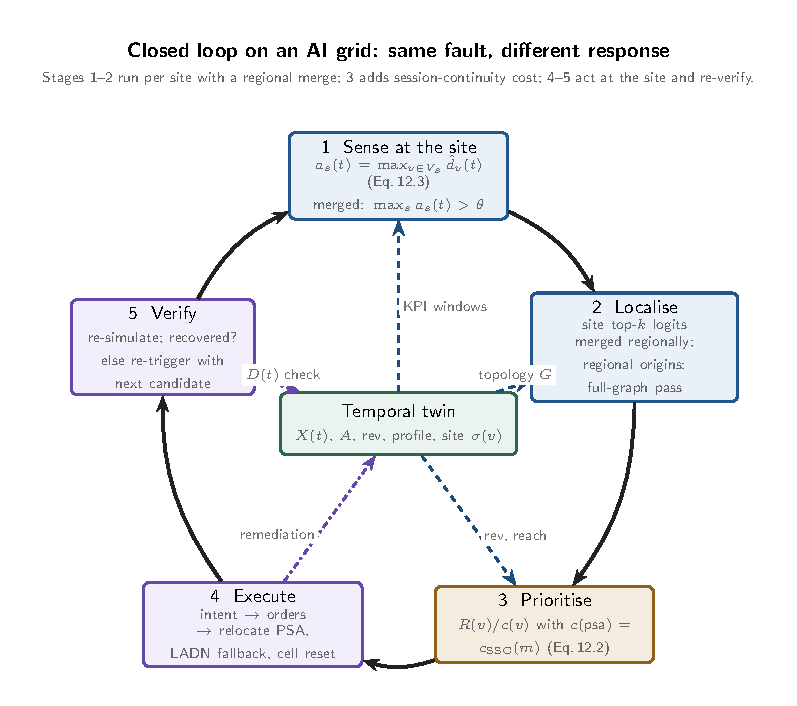
\includegraphics[width=0.78\textwidth]{../design/closed_loop.pdf}
\caption{Five stages around a twin. The only input is the KPI stream; the only output is an
ordered set of per-domain actions. Stages 1--2 are the learned model, stage 3 a one-line rule,
stages 4--5 plumbing and verification.}
\end{figure}

\section{Decomposition}
An intent with $n$ ordered targets decomposes into $n$ service orders, one per target, each
carrying the domain (RAN, Core, Transport), the target node and the remediation operation. In the
repository the intent is TMF921-shaped and the orders are TMF641-shaped: the field names follow
the standards so that a real orchestrator could be substituted for the mock, but we do not claim
conformance to either specification. The mock orchestrator records each order and returns the
step at which the highest-priority action takes effect.

\section{Measuring the loop}
The twin makes the loop measurable. We re-simulate the same fault with the injection removed from
the effective remediation step onward and record the recovery time, and we integrate the
revenue-weighted degradation over the episode:
\begin{equation}
\mathrm{Loss}=\sum_{t}\sum_{u\in\V}\mathrm{rev}_u\,d_u(t).
\label{eq:exposure}
\end{equation}
Comparing \eqref{eq:exposure} for a GNN-timed remediation against a threshold-timed one turns the
lead time of Chapter~\ref{ch:detection} into a business number on the same twin. If the model's
top-ranked origin is wrong, the remediation is applied to the wrong node, the injection is not
removed, and the GNN-timed loss is \emph{not} reduced; the metric therefore penalises wrong
root causes rather than rewarding confident ones.

\chapter{Experiments}
\label{ch:experiments}

Every number below is produced by \code{make pipeline} from a fixed seed and rendered into this
chapter by \code{scripts/results\_to\_tex.py}. Change an equation, change the module, rerun, and
the table changes.

\section{Protocol}
A single synthetic twin (Chapter~\ref{ch:domain}) is generated. Episodes of $T$ steps are
simulated; a fraction are nominal, the rest carry one fault drawn from the catalogue of
Chapter~\ref{ch:propagation} with a random origin of the matching type, a random onset in
$[T/4,T/2)$, and a random severity and ramp. Episodes are split 60/15/25 into train, calibration
and test. The model of Chapter~\ref{ch:symmetry} is trained with the loss \eqref{eq:loss}.
Every detector, the GNN field detector \eqref{eq:detection}, the service-layer $z$-score trigger,
and the per-node rolling $z$-score, is calibrated on the \emph{same} nominal calibration episodes
with the same margin, so each has zero false alarms on calibration data by construction. The
static threshold is fixed at $2.5$ standardised units.

Metrics (Chapter~\ref{ch:closed} and below): a detector's delay is the first firing at or after
onset; a firing before onset is counted as a false alarm. Lead time is reported only over episodes
where the baseline fired, and the detection-rate gap is reported separately.
\begin{align}
\text{lead}&=t_{\text{baseline}}-t_{\text{gnn}} \label{eq:leadtime}\\
\text{hit@}k&=\ind{v_0\in\text{top-}k\text{ of the ranking at }t_{\text{gnn}}+\delta} \label{eq:hitk}\\
\text{triage@}k&=1-\frac{k}{|\{u:\ d_u(t_{\text{alarm}}+\delta)>0.5\}|} \label{eq:triage}
\end{align}
The triage denominator is the set of nodes that are actually degraded when a static alarm would
have fired: the set a war room would face. Exposure is \eqref{eq:exposure} integrated over the
episode, with the remediation applied at the GNN-timed step through the verify-and-re-trigger loop,
or at the threshold-timed step.

\section{Results}
\begin{center}\small\begin{tabular}{@{}p{9.2cm}r@{}}\toprule Metric & Value \\ \midrule
Fault episodes / nominal episodes & 33 / 7 \\
Detection rate: GNN / static threshold & 1.00 / 0.97 \\
Detection rate: service $z$ (calibrated $z=4.9$ / textbook $z=3$) & 0.03 / 0.58 \\
Detection rate: per-node $z$ (calibrated $z=7.9$ / textbook $z=3$) & 0.00 / 1.00 \\
False alarms on nominal: GNN / thr. / service $z$ cal. / service $z{=}3$ / node $z$ cal. / node $z{=}3$ & 0 / 0 / 0 / 1 / 0 / 7 \\
Pre-onset false alarms on fault episodes, same order & 1 / 0 / 0 / 4 / 0 / 33 \\
Detection delay after onset (steps): GNN / static threshold & 21.6 / 35.8 \\
Detection delay (steps): service $z$ cal. / $z{=}3$; node $z$ cal. / $z{=}3$ & 38.0 / 58.6; -- / 6.9 \\
Lead time of GNN vs static threshold (steps, where it fired) & 14.2 \\
Lead time of GNN vs service $z$ (calibrated / $z{=}3$) & 18.0 / 37.2 \\
Lead time of GNN vs per-node $z$ (calibrated / $z{=}3$) & -- / -14.6 \\
Root cause hit@1 / hit@3 & 1.00 / 1.00 \\
Healed within 3 verify-and-re-trigger cycles / mean cycles & 1.00 / 1.00 \\
War-room set at alarm time (nodes) / triage reduction@3 & 15.9 / 0.33 \\
Revenue-weighted exposure: GNN-timed / threshold-timed healing & 334.2 / 815.8 \\
\bottomrule\end{tabular}\end{center}

\begin{center}\small\begin{tabular}{@{}lrrrrrr@{}}\toprule
Fault type & $n$ & delay GNN & delay thr. & delay service $z{=}3$ & hit@1 & hit@3 \\ \midrule
amf signaling storm & 9 & 25.6 & 50.2 & 58.0 & 1.00 & 1.00 \\
fiber degrade & 6 & 22.2 & 35.5 & 42.0 & 1.00 & 1.00 \\
ladn dn degrade & 1 & 20.0 & 25.0 & 31.0 & 1.00 & 1.00 \\
psa overload & 3 & 20.3 & 23.3 & 15.0 & 1.00 & 1.00 \\
router congestion & 5 & 20.4 & 35.0 & 72.0 & 1.00 & 1.00 \\
sleeping cell & 2 & 15.0 & 18.0 & 92.0 & 1.00 & 1.00 \\
upf overload & 7 & 19.4 & 32.1 & 66.8 & 1.00 & 1.00 \\
\bottomrule\end{tabular}\end{center}
\noindent\textit{Twin: 93 nodes, 198 edges. Detection threshold $\theta=0.665$. Config: episodes=160, epochs=30, T=160, window=8, seed=0. Runtime 1605.0\,s on CPU.}


\section{Reading the table}
\begin{itemize}[nosep]
  \item \textbf{Lead time.} The quantity the industry calls silent-degradation lead time is the
  GNN-versus-static-threshold row. Positive is earlier. The per-node $z$-score row is the honest
  comparison with a cheap statistical detector calibrated to the same false-alarm budget.
  \item \textbf{Root cause.} hit@1 is the fraction of episodes where the single top-ranked node is
  the injected origin, across all three domains in one softmax.
  \item \textbf{Healing cycles.} Because a remediation only removes the injection at the true
  origin, a wrong top-1 costs a cycle. The healed-within-3 rate is the end-to-end success of the
  loop, not of the model alone.
  \item \textbf{Exposure.} Revenue-weighted degradation integrated over the episode. The ratio of
  the two exposure numbers is the business version of the lead time.
\end{itemize}

\section{What would change these numbers}
The twin is small and the fault model is simple; both are the first things to vary. Longer ramps
widen the GNN's advantage; stronger coupling $\beta$ narrows it because symptoms reach the service
layer sooner. More node types and more relations make hit@1 harder. Real KPI history replaces
\eqref{eq:nominal} and will be less forgiving than AR(1) noise. None of these change the equations.

\chapter{The NVIDIA path to scale}
\label{ch:nvidia}

Everything above runs full-batch on a 74-node twin on a laptop CPU in under two minutes. An
operator's twin has $10^5$--$10^7$ nodes and the same number of KPI windows per step. The
mathematics does not change; the execution does. We assume NVIDIA hardware and the RAPIDS
ecosystem for the scaled deployment and document the path here. The repository's
\code{docs/nvidia.md} carries the installation and versioning detail.

\section{What changes mathematically: sampling}
Full-batch evaluation of \eqref{eq:rgcn} touches every edge every step. At scale one evaluates
the layer on a sampled neighbourhood~\cite{hamilton2017}: for each seed node, draw $f_\ell$
neighbours per relation at hop $\ell$ and replace the mean over $\N_r(v)$ with the mean over the
sample. The sampled aggregation is an unbiased estimate of the full one, and
\eqref{eq:equivariance} still holds in distribution because the sampler is itself index-blind.
What one loses is the exact $L$-hop receptive field; what one gains is a cost that depends on the
fan-out $f_1 f_2\cdots f_L$ and the batch, not on $N$.

\section{Where the pieces run}
\begin{itemize}[nosep]
  \item \textbf{Graph structure and features in GPU memory.} WholeGraph holds the edge list and
  the KPI window tensor across GPUs (and across nodes of a DGX system over NVLink/NVSwitch), so
  sampling and gathering never cross to host memory. This is the twin's \emph{in-memory} form; a
  durable graph store still owns history and versioning.
  \item \textbf{Sampling and gathering.} cuGraph-PyG implements PyTorch Geometric's
  \code{GraphStore}/\code{FeatureStore} and a GPU \code{NeighborLoader}. The same \code{HealingGNN}
  class consumes its mini-batches; \code{gnn/scale.py} is the adapter.
  \item \textbf{Data preparation.} cuDF replaces pandas for building the node and edge tables and
  the rolling KPI windows at scale.
  \item \textbf{Training.} PyTorch on CUDA; multi-GPU via distributed data parallel with the
  sampler sharded by seed nodes. Relational convolution kernels are the stock PyG ones; NVIDIA's
  accelerated message-passing kernels are picked up when installed.
\end{itemize}

\section{What we did and did not verify}
The CPU reference path is exercised by the test suite and the pipeline. The cuGraph-PyG and
WholeGraph path is \emph{documented and import-guarded}, not exercised in this repository's CI,
because the public release is built and tested on a machine without an NVIDIA GPU. A reader with
a CUDA 12 Linux host can install the pinned RAPIDS release and run the same pipeline with the
adapter; we state this plainly rather than imply a scale result we have not measured.

\chapter{Relation to the industry design}
\label{ch:industry}

Public material from a 2026 TM~Forum Moonshot Catalyst on business-aware GNN healing
(C26.0.965) describes a production-grade system of the same shape as this repository. We built
ours independently from the blueprint, then compared. The comparison is useful in both directions:
it shows which parts of the industry system are mathematics that anyone can reproduce, and it
shows what we deliberately left out.

\section{Stage by stage}
\begin{center}\small
\begin{tabular}{@{}p{2.2cm}p{5.8cm}p{6.2cm}@{}}
\toprule
Stage & Industry design & This repository \\
\midrule
Trigger & Service-layer $z$-score against a clean multi-week baseline with a confirmation gate; the GNN does not detect. &
Same service-layer trigger implemented as a baseline (\code{service\_zscore\_trigger}); the GNN degradation field \eqref{eq:detection} is offered as a graph-aware alternative and measured against it. \\[2pt]
Localise & Link prediction: anomaly nodes live in the property graph and the model scores ``originates-from'' edges, traversed in reverse from symptoms to origin. &
Node scoring with a softmax over all nodes \eqref{eq:rca}. Equivalent for a single incident (Remark~\ref{rem:linkpred}); transposed relations in \eqref{eq:rgcn} are the reverse traversal. \\[2pt]
Prioritise & Utility $=$ profile weight $\times$ revenue-density index $\times$ service impact, banded into a priority; a change-risk concurrency policy executes one major change at a time. &
$R(v)=\sum_u w_u\,\mathrm{rev}_u\,\hat d_u$ over the blast radius, divided by resource cost, under a budget with one change per domain \eqref{eq:selection}. Their utility is the single-node special case. \\[2pt]
Execute & TMF921 v5 healing intent decomposed into TMF641 v5 service orders, executed by a vendor orchestration engine. &
TMF921- and TMF641-shaped objects (field names, not conformance) executed by a mock orchestrator against the simulator. \\[2pt]
Verify & A reflection stage re-runs inference, reports complies/degrades, re-triggers without human escalation. &
Re-simulation with the remediation applied; if the field does not recover, re-trigger with the next ranked candidate \eqref{eq:exposure}. \\[2pt]
Training data & A 13-stage schema-faithful generator: scripted temporal arcs, domain-specific signal fingerprints, topology-driven blast radii, root-cause vs symptom labels. &
A diffusion model on the causal graph \eqref{eq:propagation} with type-specific effect vectors \eqref{eq:observation}; origin and latent field as labels. Less schema fidelity, more physics. \\[2pt]
Scale substrate & A managed temporal graph database and a managed GNN training service. &
NVIDIA path: WholeGraph, cuGraph-PyG, cuDF (Chapter~\ref{ch:nvidia}); durable store left to the reader. \\
\bottomrule
\end{tabular}
\end{center}

\section{What transfers and what does not}
Everything in the Trigger, Localise, Prioritise and Verify rows is mathematics and is in this
repository with tests. The Execute row is plumbing that any orchestrator can provide. The two
things the industry system has that this repository does not are a production-identical schema for
its synthetic corpus, which makes fine-tuning on real incidents a no-translation step, and the
standards contributions themselves (an intent-ontology extension, a new assessment questionnaire,
a proposed lead-time indicator). Neither affects the claim of Chapter~\ref{ch:claim}; both matter
for deployment.

\section{One honest difference in the detection story}
The industry trigger is a service-layer statistic. That is a sensible production choice: it is
cheap, explainable, and needs no labels. Our results (Chapter~\ref{ch:experiments}) test whether a
graph-aware detector fires earlier on the same episodes with the same calibrated false-alarm
budget, because it reads the \emph{pattern across neighbours} rather than a single node's
deviation. That is an extension of the industry design, not a replication of it, and we report it
as such, including the cases where it does not win.

\chapter{The edge: LADN, session anchors, and the AI grid}
\label{ch:edge}

Everything so far treats the twin as one graph evaluated in one place. Operators do not run one
place. Radio sites, aggregation points and metro hubs are where the KPIs are produced, and
NVIDIA's AI-grid programme puts accelerated compute at exactly those points, shared with the
AI-RAN baseband. This chapter adds the edge to the twin as structure, not as deployment detail,
and measures what evaluating the model \emph{per site} costs.

\section{Two 3GPP constructs as graph structure}
A PDU session is anchored at a UPF, the \emph{PDU Session Anchor} (PSA), which terminates N6
toward a data network. For edge traffic the PSA sits at the site behind an intermediate UPF
(I-UPF) on N9. A \emph{Local Area Data Network} (LADN) is a data network reachable only inside a
service area, a list of tracking areas, and is the normal home of enterprise, venue and MEC
applications. Both become node types, with relations oriented as before in the direction a fault
propagates:
\begin{equation}
\Tset_{\text{edge}}=\Tset\cup\{\textsf{iupf},\textsf{psa},\textsf{ladn}\},\qquad
\Rel_{\text{edge}}=\Rel\cup\{\textsf{core}\!\to\!\textsf{iupf},\ \textsf{iupf}\!\to\!\textsf{psa},\ \textsf{agg}\!\to\!\textsf{psa},\ \textsf{smf}\!\to\!\textsf{psa},\ \textsf{psa}\!\to\!\textsf{ladn},\ \textsf{cell}\!\to\!\textsf{ladn},\ \textsf{ladn}\!\to\!\textsf{service}\}.
\label{eq:edge-domain}
\end{equation}
Every node also carries a site index $\sigma(v)\in\{-1,0,\dots,S-1\}$, with $-1$ for regional
nodes (core routers and their links, I-UPF, AMF, SMF, central UPFs and their services). A PSA's
blast radius is, by construction, confined to its own site plus regional nodes: the structure
says where a session-anchor fault can and cannot be felt, and the business layer inherits that.

\begin{figure}[h]
\centering
\begin{tikzpicture}[x=1cm, y=1cm, >=Latex,
  n/.style={draw, rounded corners=2pt, minimum width=17mm, minimum height=6.5mm, font=\small, thick, fill=white},
  ran/.style={n, draw=ran, fill=ran!8}, tra/.style={n, draw=tra, fill=tra!8},
  core/.style={n, draw=core, fill=core!10}, svc/.style={n, draw=svc, fill=svc!8},
  edge/.style={n, draw=black!70, fill=black!6},
  e/.style={->, thick, draw=ink!70}, lab/.style={font=\scriptsize, fill=white, inner sep=1pt}
]
\node[tra]  (rc)   at (0, 3)     {router (core)};
\node[core] (iupf) at (3.5, 3)   {iupf};
\node[core] (smf)  at (10.5, 3)  {smf};
\node[tra]  (ra)   at (0, 1)     {router (agg)};
\node[edge] (psa)  at (3.5, 1)   {psa (site $s$)};
\node[ran]  (gnb)  at (0, -1)    {gnb};
\node[ran]  (cell) at (0, -3)    {cell};
\node[edge] (ladn) at (3.5, -1)  {ladn (site $s$)};
\node[svc]  (es)   at (7, -1)    {edge service};
\node[edge, dashed] (psab) at (10.5, 1) {psa (site $s{+}1$)};
\draw[e] (rc) -- (iupf) node[lab, midway, above] {feeds};
\draw[e] (iupf) -- (psa) node[lab, midway, left] {N9};
\draw[e] (smf.south) -- ++(0,-0.55) -- ++(-6.1,0) node[lab, pos=0.8, above] {controls} -- (psa.north east);
\draw[e] (rc) -- (ra) node[lab, midway, right] {feeds};
\draw[e] (ra) -- (psa) node[lab, midway, above] {feeds};
\draw[e] (ra) -- (gnb) node[lab, midway, right] {backhauls};
\draw[e] (gnb) -- (cell) node[lab, midway, right] {serves};
\draw[e] (psa) -- (ladn) node[lab, midway, right] {N6};
\draw[e] (cell) -- ++(1.6,0) -- (ladn.south west) node[lab, pos=0.3, below] {in service area};
\draw[e] (ladn) -- (es) node[lab, midway, above] {serves};
\draw[->, thick, dashed, draw=core!80!black] (psa.east) -- ++(0.4,0) -- ++(0,0.5) -- ++(5.2,0) node[lab, pos=0.45, above] {relocate sessions (SSC mode 3)} -- (psab.north west);
\begin{scope}[on background layer]
\node[draw=black!40, dashed, rounded corners=6pt, fit=(ra)(psa)(gnb)(cell)(ladn)(es), inner sep=7pt,
      label={[font=\scriptsize, text=black!55]below:site $s$: owned nodes; regional nodes above are its one-hop boundary}] {};
\end{scope}
\end{tikzpicture}
\caption{One edge site in the extended twin \eqref{eq:edge-domain}. The PSA and LADN are owned by
the site; the core router, I-UPF and SMF are regional and appear in the site's subgraph only as
boundary context. The dashed relocation is a remediation action, not a propagation edge.}
\end{figure}

\section{Session continuity as remediation cost}
The remediation for a degraded anchor is to re-anchor its sessions at a backup PSA, here the next
site's. How expensive that is depends on the Session and Service Continuity mode of the sessions:
mode~3 establishes the new anchor before releasing the old (make-before-break), mode~2 releases
first, mode~1 does not relocate at all. The business layer of Chapter~\ref{ch:intent} already has
the right slot: the resource cost $c(v)$ in \eqref{eq:selection} becomes mode-dependent,
\begin{equation}
c(\textsf{psa})=c_{\mathrm{SSC}}(m),\qquad c_{\mathrm{SSC}}(3)<c_{\mathrm{SSC}}(2)<c_{\mathrm{SSC}}(1),
\label{eq:ssc}
\end{equation}
so the same anchor fault at a mode-3 site is sequenced ahead of the same fault at a mode-1 site
when revenue at risk is equal. Same fault, different response, now on a 3GPP axis.

\section{Per-site inference as a graph cut}
Let $V_s=\{v:\sigma(v)=s\}$ be the nodes a site owns and $B_s$ its one-hop boundary in either
direction of $\Rel'$. The site evaluates the \emph{same} network of Chapter~\ref{ch:symmetry} on
the induced subgraph $G[V_s\cup B_s]$ and reports a summary,
\begin{equation}
a_s(t)=\max_{v\in V_s}\hat d_v(t),\qquad
Z_s(t)=\text{top-}k\big\{(v,z_v(t)):\ v\in V_s\cup B_s\big\},
\label{eq:site-summary}
\end{equation}
and the regional merge is $a(t)=\max_s a_s(t)$ with the ranking taken over the union of the
$Z_s(t)$, each node scored by the best site that saw it. Per step a site uplinks $1+2k$ scalars
instead of $|V_s|\cdot K$ KPI values; the KPI windows never leave the site.

What is lost is exact: a node's $L$-hop receptive field is truncated at the cut. For a site-owned
origin the cut removes only distant context, and the experiment shows no loss. For a regional
origin, a core router or the I-UPF, no site owns the node and each site sees only its symptoms;
the per-site ranking then names the site's boundary copy of the regional node, or a symptomatic
owned node. That is the partition's cost, and it is the reason the design keeps a full-graph pass
at the metro hub for regional-origin faults. The table in Chapter~\ref{ch:experiments} on this
branch reports hit@1 separately for site-local and regional origins.

\section{Where the serving stack goes}
The GNN is small and latency-bound, not throughput-bound: it belongs under a standard inference
server at the site, on the GPU the AI-RAN baseband already occupies. NVIDIA Dynamo is the wrong
tool for the GNN and the right tool for the reasoning agents around it. The industry design wraps
the five stages in LLM agents; on an AI grid those agents are an OpenAI-compatible service whose
long shared context (topology, intent vocabulary, standards payload templates) is prefilled once
at the hub and whose per-incident decoding runs on the smaller site GPUs, with Dynamo's KV-aware
router keeping each site's agent warm for its own topology and NIXL moving KV state across the
grid fabric. \code{docs/edge-ai-grid.md} and \code{deploy/ai-grid/} describe the shape; neither
is exercised in this repository, and we say so.

\appendix
\chapter{Equation-to-code map}
\label{app:map}
\begin{figure}[h]
\centering
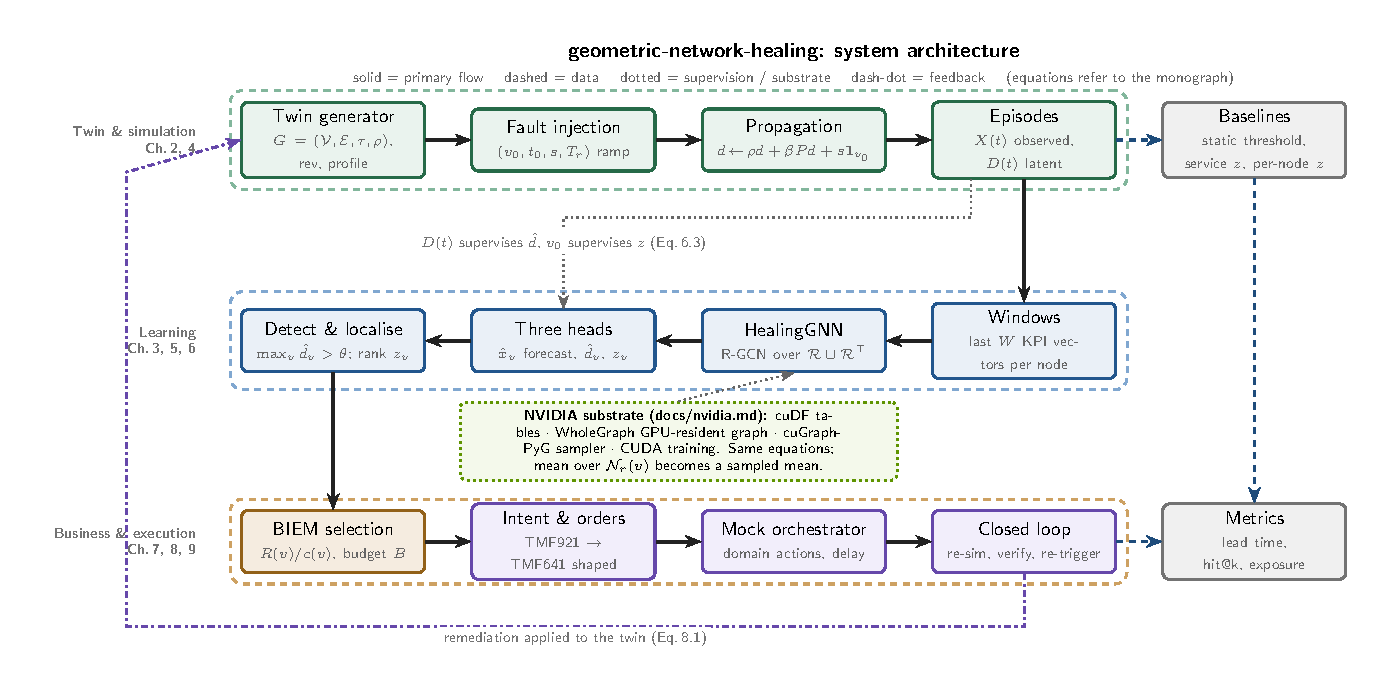
\includegraphics[width=\textwidth]{../design/architecture.pdf}
\caption{System architecture of the repository. Equation numbers refer to this document.}
\end{figure}
\begin{center}
\small
\begin{tabular}{@{}llp{7.2cm}@{}}
\toprule
Equation & Module & Symbol \\
\midrule
\eqref{eq:graph}, \eqref{eq:adjacency}, \eqref{eq:signal} & \code{twin/schema.py}, \code{twin/generator.py} & \code{NodeType}, \code{Relation}, \code{Twin.adjacency()}, \code{Twin.to\_pyg()} \\
\eqref{eq:revenue} & \code{twin/generator.py} & \code{nodes["revenue"]}, \code{Twin.downstream()} \\
\eqref{eq:action}, \eqref{eq:equivariance} & \code{tests/test\_model.py} & numerical equivariance check \\
\eqref{eq:mp}, \eqref{eq:rgcn}, \eqref{eq:input}, \eqref{eq:heads} & \code{gnn/model.py} & \code{HealingGNN} \\
\eqref{eq:injection} & \code{sim/faults.py} & \code{Fault.injection()} \\
\eqref{eq:nominal}, \eqref{eq:observation}, \eqref{eq:propagation} & \code{sim/dynamics.py} & \code{simulate()} \\
\eqref{eq:stability} & \code{tests/test\_twin\_and\_sim.py} & \code{test\_faults\_attenuate\_per\_hop} \\
\eqref{eq:alarm} & \code{baselines/alarms.py} & \code{threshold\_alarm\_detection()}, \code{zscore\_detection()} \\
\eqref{eq:residual}, \eqref{eq:detection} & \code{gnn/detect.py} & \code{calibrate\_threshold()}, \code{detect()} \\
\eqref{eq:forward} & \code{sim/dynamics.py} & implicit in the recursion \\
\eqref{eq:rca} & \code{gnn/detect.py} & \code{rank\_root\_causes()} \\
\eqref{eq:loss} & \code{gnn/train.py} & \code{train()} \\
\eqref{eq:rar}, \eqref{eq:selection} & \code{intent/biem.py} & \code{propose\_branches()}, \code{select\_order()}, \code{to\_tmf921\_intent()} \\
\eqref{eq:exposure} & \code{orchestration/tmf641.py} & \code{closed\_loop()} \\
\eqref{eq:leadtime}--\eqref{eq:triage} & \code{evaluation/metrics.py} & \code{lead\_time()}, \code{hit\_at\_k()}, \code{triage\_reduction()} \\
sampling (Ch.~\ref{ch:nvidia}) & \code{gnn/scale.py} & \code{make\_cugraph\_loader()} \\
\bottomrule
\end{tabular}
\end{center}

\chapter{Reproducing every number}
\label{app:repro}
\begin{lstlisting}
git clone https://github.com/dkypuros/geometric-network-healing
cd geometric-network-healing
make setup          # uv venv, CPU PyTorch + PyG
make test           # 6 tests incl. the equivariance check
make pipeline       # twin -> simulate -> baselines -> GNN -> intent -> closed loop
cat results/results.md
make pdf            # this document
\end{lstlisting}
The pipeline is seeded; \code{--seed} changes the twin, the episodes and the initialisation
together. \code{--episodes}, \code{--epochs}, \code{--T}, \code{--window}, \code{--budget} are the
knobs most worth turning. On a CUDA host, \code{make setup-nvidia} adds the RAPIDS stack and
\code{gnn-healing backend} reports what was detected.


\begin{thebibliography}{9}
\bibitem{bronstein2021} M.~M. Bronstein, J.~Bruna, T.~Cohen, P.~Veli\v{c}kovi\'c.
\emph{Geometric Deep Learning: Grids, Groups, Graphs, Geodesics, and Gauges}. arXiv:2104.13478, 2021.
\bibitem{schlichtkrull2018} M.~Schlichtkrull et al. \emph{Modeling Relational Data with Graph Convolutional Networks}. ESWC 2018.
\bibitem{hamilton2017} W.~Hamilton, R.~Ying, J.~Leskovec. \emph{Inductive Representation Learning on Large Graphs}. NeurIPS 2017.
\bibitem{xu2019} K.~Xu, W.~Hu, J.~Leskovec, S.~Jegelka. \emph{How Powerful are Graph Neural Networks?} ICLR 2019.
\bibitem{fey2019} M.~Fey, J.~E. Lenssen. \emph{Fast Graph Representation Learning with PyTorch Geometric}. ICLR-W 2019.
\bibitem{tmf921} TM~Forum. \emph{TMF921 Intent Management API} and \emph{TMF641 Service Ordering API}; \emph{Intent Ontology (TIO)}.
\bibitem{rapids} NVIDIA. \emph{RAPIDS cuGraph, cuGraph-PyG, WholeGraph} documentation.
\end{thebibliography}
\end{document}
